\newpage
\section{Distribution block}
\label{sec:SMPS}
A conversion from the 48V to a supply voltage 5V is needed to supply various parts of the circuit. Therefore it is required to use a DC-DC converter for the conversion. It has been chosen by the designer that the converter is being implemented as a switch mode power supply (SMPS from here and onwards). This is chosen as the efficiency of SMPS is increasingly higher than others converters e.g. LDO's. The downside to using a SMPS is that additional components must be used.  

\subsection{Design}

When designing SMPS there is several packages out there, that works with passive componentes only. These packages makes the job for the designer much easier as many of the considerations are made for you. Considerations that still much be taken into account are input and output voltages, which already have been decided here. The next thing that can be considered is the efficiency of the package, which is stated in the datasheet.

It has been chosen to use the LT8300 Isolated Flyback Converter from Linear Technology. The implementation is done almost according to the datasheet(see figure \vref{fig:LT8300}) \cite{LT8300} except there is implemented a snubbercircuit and a decoupling capacitor before the transformer. Furthermore the values of the resistors are changed.  \\

\begin{figure}[H]
	\centering
	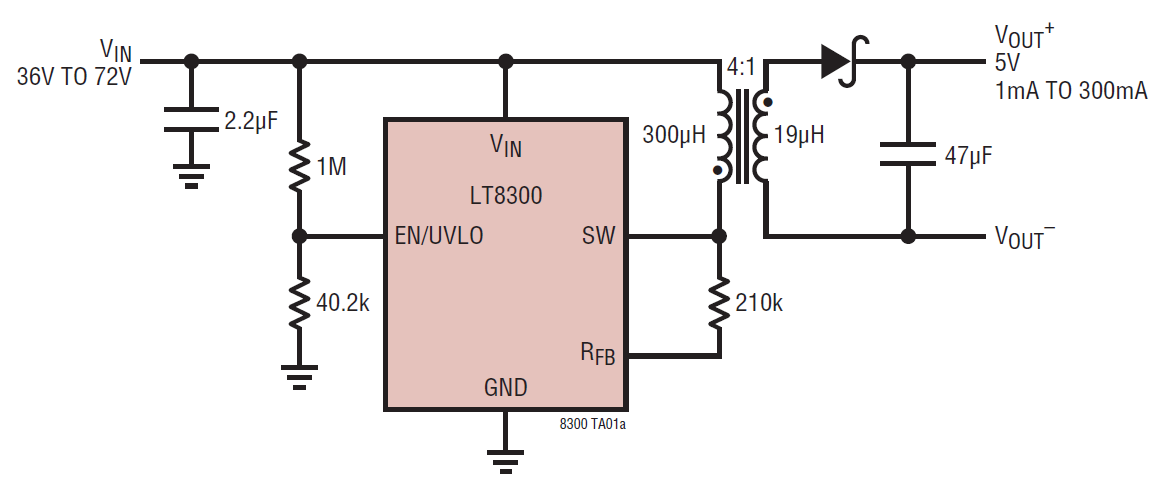
\includegraphics[width=0.6\linewidth]{Hardware/Pictures/LT8300_circuit}
	\caption{Circuit from LT8300 datasheet}
	\label{fig:LT8300}
\end{figure}

\subsection{Implementation}

Figure \vref{fig:SMPS_control} shows the hardware implementation of the SMPS. There is implemented some form of protection circuit before the signal comes into the actual SMPS. This is done by a fuse that limits the current running into the SMPS. 

\begin{figure}[H]
	\centering
	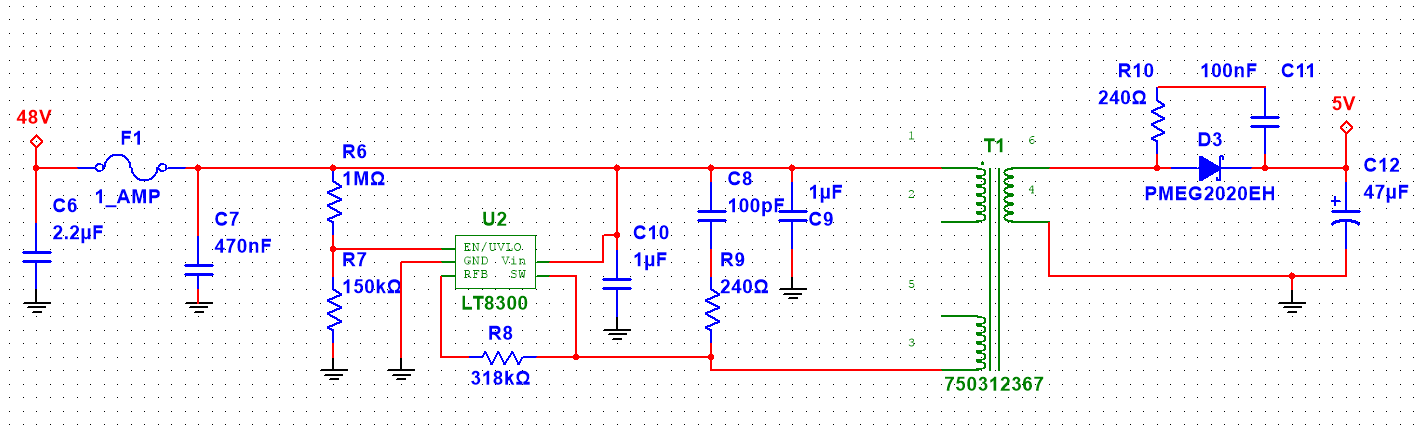
\includegraphics[width=0.7\linewidth]{Hardware/Pictures/SMPS_hw}
	\caption{Step down converter hardware overview}
	\label{fig:SMPS_control}
\end{figure}

There are various resistors can be changed and thereby change the different things e.g. the output voltage. 

The value of the resistor R8 on figure \vref{fig:SMPS_control} is calculated on the formula below. The value of this resistor decides the output of the SMPS.

\begin{align}
	\begin{split}
		R_{FB} &= \frac{N \cdot (V_{out}+V_F)}{\SI{100}{\micro \ampere}}
	\end{split}
\end{align}

Where:\\
N is the number of turns on the primary inductor. Here 6 is used. \\
$V_{out}$ is the desired output voltage from the SMPS. This is chosen to be 5V. \\
$V_F$ is the forward voltage of the diode in output stage. This is set 0.3V as a schottkey is used. \\
$R_{FB}$ is the feedback resistor. \\
This calculation yields a resistance of 318 k$\Omega$.

The dimensions of the snubber circuits are standard sizes. Furthermore, there is used decoupling capacitors to reduce the ripple on the output and to ensure a steady current for the IC.

\subsection{Unity test}
There have been tested extensively on this module. All the tests have come up with at negative response.

The test is done by placing the a voltage source, either batteries or a voltage generator supplying 48V. Then measurements were made on the secondary side of the transformer, where output should be 5V. These test were non-succesful as no voltage was coming through the transformer and therefore the desired effect of this module fails to deliver. As this is very vital part on the PCB, as this is the supply voltage for all the modules. It has therefore had an extremely large priority in getting the enitre PCB up and running. Even with this priority it was not possible to detect the problems with the module, but due to the importancy it is crucial to get up and running.  